\documentclass[border=3pt]{standalone}
\usepackage[T1]{fontenc}
\usepackage{lmodern,amsmath,pgfplots}
\usepgfplotslibrary{groupplots}
\pgfplotsset{compat=1.18}
\definecolor{MeanBlue}{HTML}{245D80}
\begin{document}
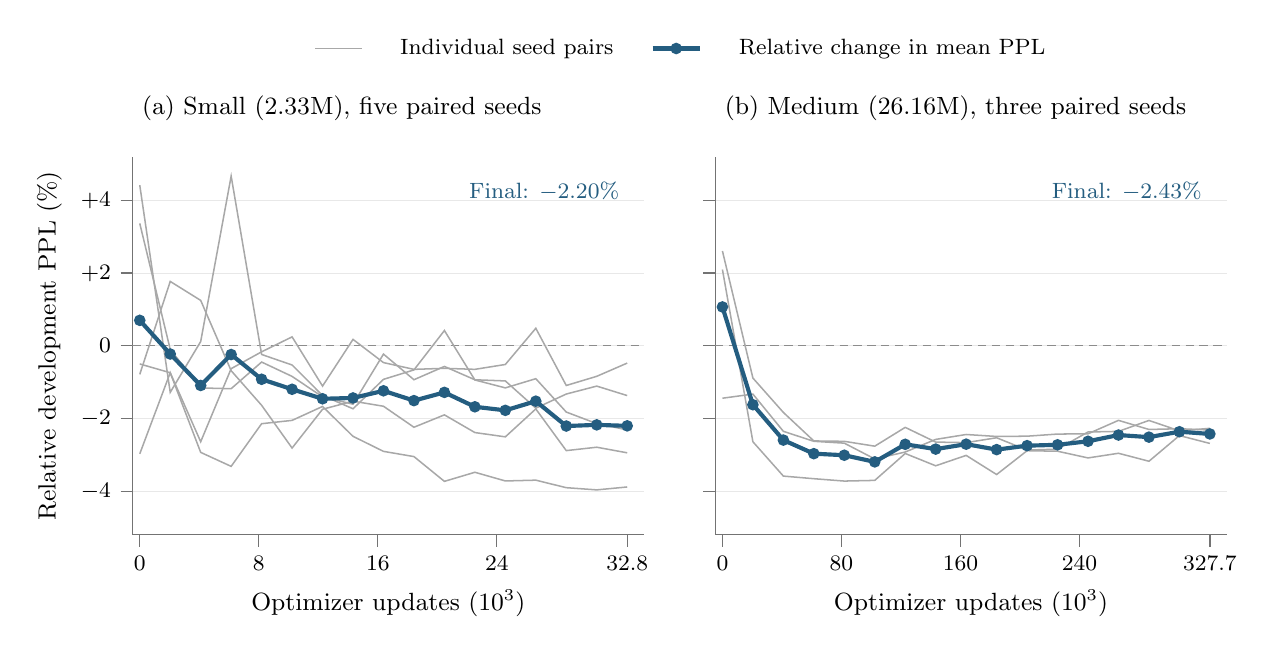
\begin{tikzpicture}
\begin{groupplot}[
group style={group size=2 by 1,horizontal sep=9mm},
scale only axis,width=65mm,height=48mm,
axis lines*=left,axis line style={black!55,line width=.45pt},
tick style={black!55,line width=.45pt},tick align=outside,
ticklabel style={font=\fontsize{8}{10}\selectfont},
label style={font=\fontsize{9}{11}\selectfont},
title style={font=\fontsize{9}{11}\selectfont,anchor=south west,at={(0,1.025)}},
ymin=-5.2,ymax=5.2,ytick={-4,-2,0,2,4},
yticklabels={$-4$,$-2$,$0$,$+2$,$+4$},
ymajorgrids=true,grid style={black!9,line width=.35pt},
scaled ticks=false,xlabel={Optimizer updates ($10^3$)},
legend style={draw=none,fill=none,font=\fontsize{8}{10}\selectfont,
at={(1.075,1.23)},anchor=south,legend columns=2,column sep=4mm},
legend cell align=left,clip=true]
\nextgroupplot[title={(a) Small (2.33M), five paired seeds},xmin=-0.491520,xmax=33.914880,xtick={0,8,16,24,32.768},xticklabels={0,8,16,24,32.8},ylabel={Relative development PPL (\%)}]
\addplot[black!45,densely dashed,line width=.5pt,forget plot] coordinates {(-0.49152,0) (33.91488,0)};
\addplot[black!34,line width=.55pt,no marks] coordinates {(0,4.41970390526) (2.048,-1.28125353572) (4.096,0.116632202821) (6.144,4.66835095684) (8.192,-0.238997536529) (10.24,-0.528734699) (12.288,-1.36737216856) (14.336,-1.73346994085) (16.384,-0.923775361541) (18.432,-0.663972621371) (20.48,0.419926051832) (22.528,-0.940606868201) (24.576,-1.15843933194) (26.624,-0.905507250558) (28.672,-1.82335432606) (30.72,-2.14188292781) (32.768,-2.31292749563)};
\addlegendentry{Individual seed pairs}
\addplot[black!34,line width=.55pt,no marks,forget plot] coordinates {(0,3.36805440938) (2.048,-0.100212077521) (4.096,-1.16072199919) (6.144,-1.18034510153) (8.192,-0.447484792773) (10.24,-0.842276269316) (12.288,-1.40616165147) (14.336,-1.60728537461) (16.384,-0.22856137615) (18.432,-0.933770813305) (20.48,-0.568333123672) (22.528,-0.935089929269) (24.576,-0.967098858567) (26.624,-1.71646912354) (28.672,-1.32784935519) (30.72,-1.10927562272) (32.768,-1.36988906737)};
\addplot[black!34,line width=.55pt,no marks,forget plot] coordinates {(0,-0.499690511575) (2.048,-0.741651630343) (4.096,-2.63982106112) (6.144,-0.629122403761) (8.192,-0.165422377551) (10.24,0.244936360413) (12.288,-1.10896423496) (14.336,0.176052241428) (16.384,-0.462310335043) (18.432,-0.648786139075) (20.48,-0.620255004336) (22.528,-0.648149451673) (24.576,-0.514542653563) (26.624,0.481565809942) (28.672,-1.09238296314) (30.72,-0.840215967901) (32.768,-0.476256699112)};
\addplot[black!34,line width=.55pt,no marks,forget plot] coordinates {(0,-2.97249016811) (2.048,-0.740940382581) (4.096,-2.93327185259) (6.144,-3.31804324087) (8.192,-2.14375478248) (10.24,-2.05269596283) (12.288,-1.66917145204) (14.336,-2.49131073487) (16.384,-2.90534838575) (18.432,-3.04882494844) (20.48,-3.73062238324) (22.528,-3.48074266983) (24.576,-3.71935191181) (26.624,-3.69786883663) (28.672,-3.90444631338) (30.72,-3.96502975419) (32.768,-3.8849355117)};
\addplot[black!34,line width=.55pt,no marks,forget plot] coordinates {(0,-0.786898566396) (2.048,1.77099186271) (4.096,1.24908054044) (6.144,-0.685541973096) (8.192,-1.63774716914) (10.24,-2.81374671365) (12.288,-1.7466602536) (14.336,-1.52415753693) (16.384,-1.66388127694) (18.432,-2.24169000402) (20.48,-1.90077191988) (22.528,-2.38758793865) (24.576,-2.50577583875) (26.624,-1.73745742941) (28.672,-2.88442249257) (30.72,-2.79104249282) (32.768,-2.9449988378)};
\addplot[MeanBlue,line width=1.5pt,mark=*,mark size=1.3pt,mark options={solid,fill=MeanBlue,draw=MeanBlue}] coordinates {(0,0.700326871209) (2.048,-0.226318424481) (4.096,-1.09231801467) (6.144,-0.240846320546) (8.192,-0.921358079549) (10.24,-1.19682739216) (12.288,-1.45836491839) (14.336,-1.4355921245) (16.384,-1.23904158559) (18.432,-1.50903271336) (20.48,-1.28229450759) (22.528,-1.67894776126) (24.576,-1.77659085604) (26.624,-1.52436829171) (28.672,-2.20796050903) (30.72,-2.1760298787) (32.768,-2.2031202124)};
\addlegendentry{Relative change in mean PPL}
\node[anchor=north east,text=MeanBlue,font=\fontsize{8}{10}\selectfont,align=right] at (rel axis cs: .97,.96) {Final: $-2.20\%$};
\nextgroupplot[title={(b) Medium (26.16M), three paired seeds},xmin=-4.915200,xmax=339.148800,xtick={0,80,160,240,327.68},xticklabels={0,80,160,240,327.7},yticklabels={}]
\addplot[black!45,densely dashed,line width=.5pt,forget plot] coordinates {(-4.9152,0) (339.1488,0)};
\addplot[black!34,line width=.55pt,no marks,forget plot] coordinates {(0,2.09849970923) (20.48,-2.64061870901) (40.96,-3.5855347014) (61.44,-3.65744165444) (81.92,-3.72248542187) (102.4,-3.7039487636) (122.88,-2.96402656931) (143.36,-3.30206726706) (163.84,-3.01598722697) (184.32,-3.54248212002) (204.8,-2.88703710223) (225.28,-2.90120391222) (245.76,-3.08592908076) (266.24,-2.95762792812) (286.72,-3.17706871154) (307.2,-2.47031874174) (327.68,-2.68678207452)};
\addplot[black!34,line width=.55pt,no marks,forget plot] coordinates {(0,2.60825892256) (20.48,-0.88804122394) (40.96,-1.83414224018) (61.44,-2.61844519332) (81.92,-2.62914578607) (102.4,-2.76230128709) (122.88,-2.24511628502) (143.36,-2.64979836672) (163.84,-2.66496920996) (184.32,-2.53084494396) (204.8,-2.8694274632) (225.28,-2.84524874209) (245.76,-2.37171473208) (266.24,-2.35572274793) (286.72,-2.05423371233) (307.2,-2.34062123817) (327.68,-2.27135209843)};
\addplot[black!34,line width=.55pt,no marks,forget plot] coordinates {(0,-1.44266620136) (20.48,-1.32898093965) (40.96,-2.35396329157) (61.44,-2.6282189775) (81.92,-2.67916755976) (102.4,-3.11411825976) (122.88,-2.92342855415) (143.36,-2.57593775175) (163.84,-2.44110510105) (184.32,-2.49487721049) (204.8,-2.48756291792) (225.28,-2.42908256544) (245.76,-2.42214088431) (266.24,-2.05202731402) (286.72,-2.30245141677) (307.2,-2.28232488894) (327.68,-2.31772932514)};
\addplot[MeanBlue,line width=1.5pt,mark=*,mark size=1.3pt,mark options={solid,fill=MeanBlue,draw=MeanBlue},forget plot] coordinates {(0,1.06892217819) (20.48,-1.62109121775) (40.96,-2.59481494008) (61.44,-2.96885154926) (81.92,-3.01157915938) (102.4,-3.19470724928) (122.88,-2.71093649963) (143.36,-2.84300970199) (163.84,-2.70734062259) (184.32,-2.85725321571) (204.8,-2.74821515641) (225.28,-2.72495180724) (245.76,-2.62744157711) (266.24,-2.45621918948) (286.72,-2.51360431275) (307.2,-2.36451555602) (327.68,-2.42580335194)};
\node[anchor=north east,text=MeanBlue,font=\fontsize{8}{10}\selectfont,align=right] at (rel axis cs: .97,.96) {Final: $-2.43\%$};
\end{groupplot}
\end{tikzpicture}
\end{document}
